%\title{LOGIC GATES}
\author{Oaboloka Bodigelo}

\section{Logic Gates}

\subsection{Introduction}

A logic gate is a device that performs a Boolean function. Each input and output of such a device can be represented as a member of the set {0,1}, where 0 typically denotes a low or false state, and 1 denotes a high or true state. Logic gates perform basic Boolean operations like AND, OR and NOT, which makes it possible to build and solve more complex logical expressions.

\subsection{Types of Gates}

\subsection*{Inverter}

The inverter gate, also called a NOT gate, takes the value of a single Boolean variable as input and produces it’s complement as output. The inverter symbol shows the input on the left and the output on the right.

\begin{figure}[H]
    \centering
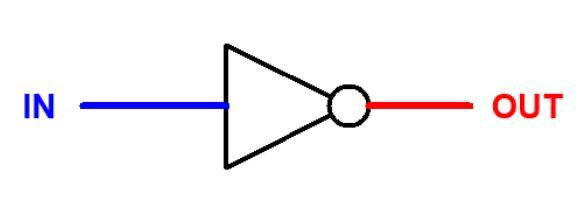
\includegraphics[width=0.5\linewidth]{images/not-gate}
    \caption{NOT gate}
    \label{fig:placeholder3}
\end{figure}

\begin{table}[H]
    \centering
    \caption*{\textbf{Truth Table: Inverter Gate}}
    \begin{tabular}{cc}
        \toprule
        $x$(IN) & $y$(OUT) \\
        \midrule
        0 & 1 \\
        1 & 0 \\
        \bottomrule
    \end{tabular}
\end{table}
 \begin{center}
 Boolean Expression: 
  x = y    
\end{center}

\subsection*{OR gate}

The OR gate that is true(1) when one or both inputs are true(1). If all OR gates are false, the output is false(0). The output is the Boolean sum of their values. The inputs are on the left and the outputs on the right.

\begin{figure}[H]
    \centering
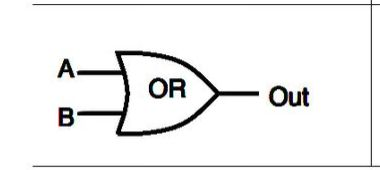
\includegraphics[width=0.5\linewidth]{images/or-gate}
    \caption{OR gate}
    \label{fig:placeholder4}
\end{figure}

\begin{table}[H]
    \centering
    \caption*{\textbf{Truth Table:OR Gate}}
    \begin{tabular}{ccc}
        \toprule
        $x$ & $y$ & $x + y$(out) \\
        \midrule
        0 & 0 & 0 \\
        1 & 0 & 1 \\
        0 & 1 & 1 \\
        1 & 1 & 1 \\
        \bottomrule
    \end{tabular}
\end{table}

\begin{center}
Boolean Expression: $A = x + y$
\end{center}

\subsection*{AND gate}

The  AND gate that is used to perform logical multiplication of input. The output of the AND gate will be true if both inputs are true(1), otherwise the output will be false(0) if any of the input is false(0). The input is shown on the left,and the output is shown on the right.

\begin{figure}[H]
    \centering
    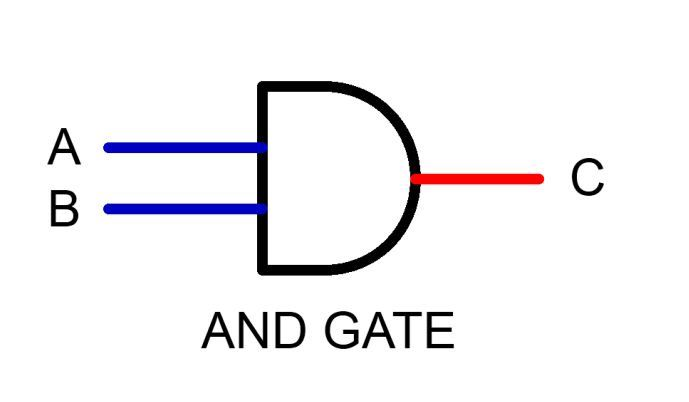
\includegraphics[width=0.5\linewidth]{images/and-gate}
    \caption{AND gate}
    \label{fig:placeholder5}
\end{figure}

\begin{table}[H]
    \centering
    \caption*{\textbf{Truth Table: AND Gate}}
    \begin{tabular}{ccc}
        \toprule
$a$ & $b$ & $a \cdot b$(c) \\
\midrule
0 & 0 & 0 \\
1 & 0 & 0 \\
0 & 1 & 0 \\
1 & 1 & 1 \\
        \bottomrule
    \end{tabular}
\end{table}

\begin{center}
Boolean Expression: $A$ = $a \cdot b$
\end{center} 

\subsection*{NAND gate}

The NAND gate, also known as negated AND, gives an output is false(0) if both inputs are true(1). The inputs are shown on the left,and the output is shown on the right.

\begin{figure}[H]
    \centering
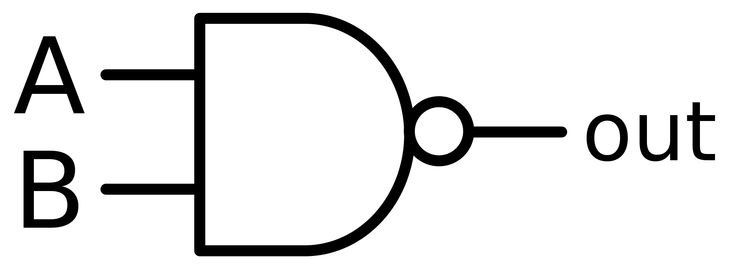
\includegraphics[width=0.5\linewidth]{images/nand-gate}
    \caption{NAND gate}
    \label{fig:placeholder6}
\end{figure}

\begin{table}[H]
    \centering
    \caption*{\textbf{Truth Table: NAND Gate}}
    \begin{tabular}{ccc}
        \toprule
  $a$ & $b$ & $\overline{ab}$'(c) \\
 \midrule
  0 & 0 & 1 \\
  0 & 1 & 1 \\
  1 & 0 & 1 \\
  1 & 1 & 0 \\
        \bottomrule
    \end{tabular}
\end{table}

\begin{center}
Boolean Expression: $A = \overline{x \cdot y}$
\end{center}

\subsection*{NOR gate}

A NOR gate is a digital circuit that gives us a true(1) output when there are false(0) input signals.

\begin{figure}[H]
    \centering
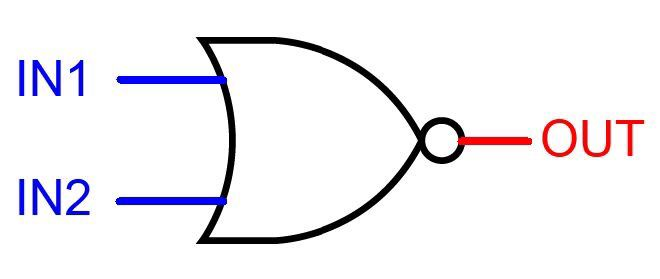
\includegraphics[width=0.5\linewidth]{images/nor-gate}
    \caption{NOR gate}
    \label{fig:placeholder7}
\end{figure}

\begin{table}[H]
    \centering
    \caption*{\textbf{Truth Table:NOR Gate}}
    \begin{tabular}{ccc}
        \toprule
         $x$ & $y$ & $\overline{x + y}$(out) \\
        \midrule
        0 & 0 & 1 \\
        0 & 1 & 0 \\
        1 & 0 & 0 \\
        1 & 1 & 0 \\
        \bottomrule
    \end{tabular}
\end{table}

\begin{center}
Boolean Expression: $A = \overline{x + y}$
\end{center}

\subsection*{XOR gate}

An XOR also known as Exclusive OR gate is a digital logic gate that outputs true(1) only when the number of inputs is odd.

\begin{figure}[H]
    \centering
    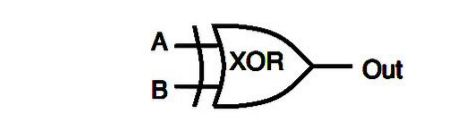
\includegraphics[width=0.5\linewidth]{images/xor-gate}
    \caption{XOR gate}
    \label{fig:placeholder8}
\end{figure}

\begin{table}[H]
    \centering
    \caption*{\textbf{Truth Table:XOR Gate}}
    \begin{tabular}{ccc}
        \toprule
        $x$ & $y$ & $x \oplus y$(out) \\
        \midrule
        0 & 0 & 1 \\
        0 & 1 & 0 \\
        1 & 0 & 0 \\
        1 & 1 & 1\\
        \bottomrule
    \end{tabular}
\end{table}

\begin{center}
Boolean expression: $A = x \oplus y$
\end{center}

\subsection{Combinations of Gates}

Combinational circuits can be built using inverters, OR gates and, the AND gates at the same time, where some gates may share inputs; this can be shown by using branching line or written separately for each gate.

steps on how to make a combinational cirucUit;

\textbf {1.} Identify the inputs and outputs of the circuit.

\textbf{2.} Draw a truth table with all possible input values that should match the output values.

\textbf{3.} Derive the Boolean expression for the circuit.

\textbf{4.} Simplify the Boolean expression using K-Map or algebraic methods

\textbf{5.} Draw  the logic diagram using the Boolean expression

For example;

\begin{figure}[H]
    \centering
    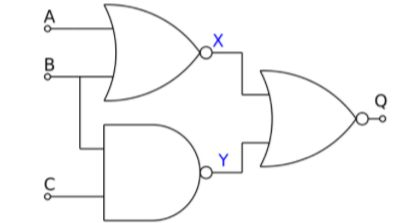
\includegraphics[width=0.5\linewidth]{images/combinational-circuit}
    \caption{Combinational circuit}
    \label{fig:placeholder9}
\end{figure}

\begin{table}[H]
    \centering
    \caption*{\textbf{Truth Table:Combinational circuit}}
    \begin{tabular}{ccccccc}
        \toprule
        $A$ & $B$ & $C$ & $X$ & $Y$ & $Z$ & $Q$\\
        \midrule
        0 & 0 & 0 & 0 & 1 & 1 & 0 \\
        0 & 0 & 1 & 0 & 1 & 1 & 0 \\
        0 & 1 & 0 & 1 & 0 & 0 & 0\\
        0 & 1 & 1 & 1 & 0 & 1 & 1\\
        1 & 0 & 0 & 1 & 1 & 1 & 1\\
        1 & 0 & 1 & 1 & 1 & 1 & 1\\
        1 & 1 & 0 & 1 & 0 & 0 & 0\\
        1 & 1 & 1 & 1 & 0 & 1 & 1\\
        \bottomrule
    \end{tabular}
\end{table}    
